



\begin{frame}{\citetitle{MarcoNuno_Revista_2020_06_00} \footnotemark (1)}
\begin{block}{Problem description} 

During pandemics, most of the parents are not used to simultaneously deal with their home office activities and the monitoring of the home school activities of their children. 
%\note[item]{The next project in my presentation is called \Titulo}
\note[item]{Therefore, a system allowing a parent, teacher or tutor to assign a task and its corresponding execution time to children, could be helpful in this situation.}


	\begin{itemize}
		\item There is not a way to monitor the attention levels of children solving assigned tasks that cannot be supervised by an adult.
		\item The monitoring information is useful for both, parents and teachers
		\item It could be useful to know the time that children spends on solving a given task.
	\end{itemize}

We propose a Remote Learning Monitoring System (RLMS) to assign academic tasks to a child, to measure the task performing time, and monitor the child's learning process.

\note[item]{The proposed tools are focused on handwritten tasks, such as solving math operations, writing text or drawing, where children do not directly interact with the smartphone or tablet, and use it only to read the task description}

\end{block} 
\footnotetext[1]{\fullcite{MarcoNuno_Revista_2020_06_00}}
\setcounter{footnote}{0}

\end{frame}


\begin{frame}{\citetitle{MarcoNuno_Revista_2020_06_00} (2)}
\begin{block}{Screens of the proposed system} 

    \begin{columns}
    \begin{column}{0.6\textwidth}  
    Components:
    \begin{itemize}
        \item Desktop App (DaLeMO).
            \begin{itemize}
            \item There are five main panels.
\note[item]{Group Management, Student Management, Activity Management, Activity Assignment Management Pannels and the most relevant, the Learning Monitoring Management Panel that allows the teacher to access basic statistics of the time of each activity and sort them by date, duration, or, completion percentage.}
            \end{itemize}        
        \item Mobile App (MaLeMO).
        \begin{itemize}
            \item Was tested on multiple devices.
            \item Displays a front camera preview.
\note[item]{This element was designed to be small and
unnoticed by the user, and provides the frames to the image processing module that analyses the student's face for estimate gaze direction and to conclude if student has attention on the current activity.}
            \item The app allows the user to start and pause the current activity.
%\note[item]{The students control the start and pause of their work by the start and pause activity buttons.}
            \item When the student finishes, the app allows the user to capture and report the activity' evidence.
%\note[item]{When the student finishes, the app allow to capture a image of the performed work.}
            
        \end{itemize}
        \end{itemize}
    
        \end{column}

    \begin{column}{0.4\textwidth}  
        \begin{center}
     %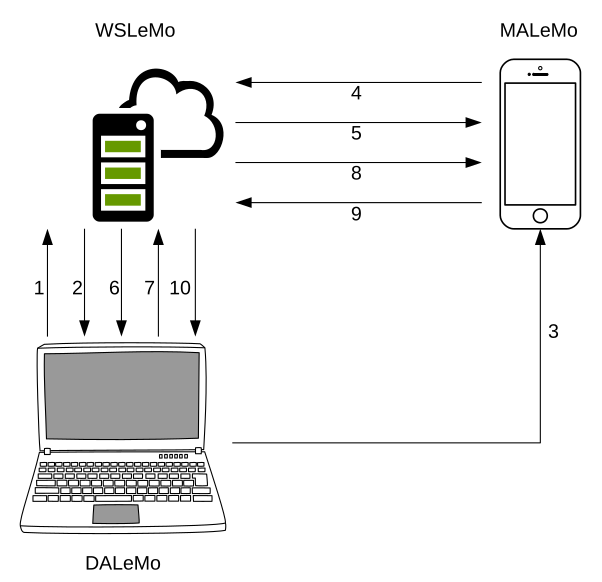
\includegraphics[width=0.75\textwidth]{Figs/LearningMonitoring5}
     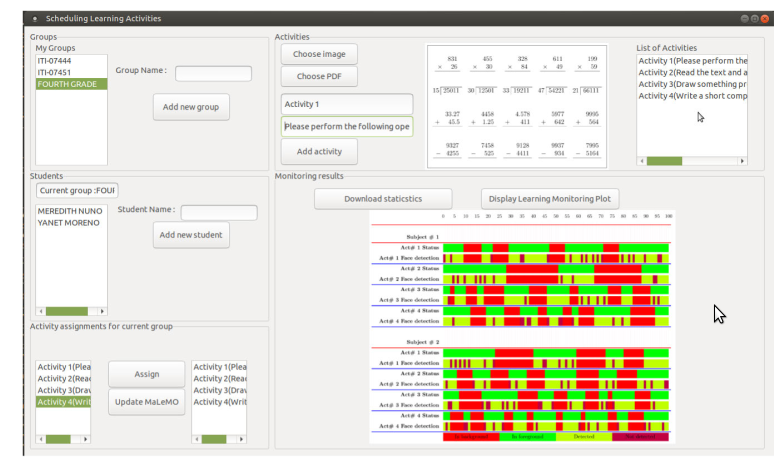
\includegraphics[width=0.85\textwidth]{Figs/LearningMonitoring1}
     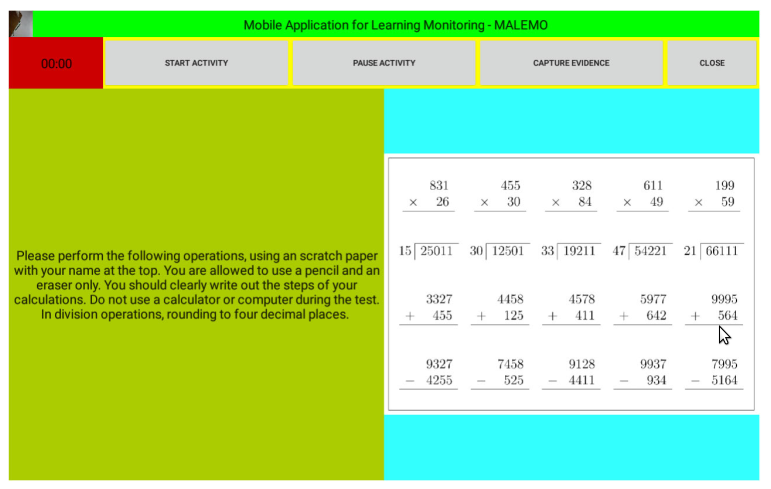
\includegraphics[width=0.85\textwidth]{Figs/LearningMonitoring2}
     \end{center}
    \end{column}
        \end{columns}
     
\end{block} 
\end{frame}



\begin{frame}{\citetitle{MarcoNuno_Revista_2020_06_00} (3)}
\begin{block}{Learning monitoring results} 

\begin{columns}
\begin{column}{0.5\textwidth}
Test environment:
		\begin{itemize}
		\item A child must be seated in front of a base holding a smartphone.
\note[item]{The Screen tilt angle must be between 45 and 85 degrees.}
\note[item]{Maximum seating distance: one meter to the device's screen}
\note[item]{No adults must be in front of or near the child when the activity is being carried out.}
		\end{itemize}
Analysis of the usage time.
		\begin{itemize}
		\item Experimentation with two different subjects performing four activities was done.
\note[item]{The activities were: Writing, reading, Drawing and Math.}
		\item Foreground or the background time of the app is measured.
\note[item]{The active time is the time the MaLeMO is kept in the foreground, while the inactive time is the time the MaLeMO is kept in the background. }		
		\item The time that monitored subject faces was detected from the camera is also measured.
\note[item]{The face analysis stage can only be performed when the
application is in the foreground.}		
\note[item]{We can measure the frame percentage with a missing face and Net Attention Time from frames with detected faces. }
		\end{itemize}

%In this work, a Remote Learning Monitoring Systems (RLMS) has been proposed. The proposed systems allow the parent or teacher to use the DaLeMO to assign some learning activities to be carried out by children. Children can use the MaLeMO to read the instructions of these activities, and remotely send image-based evidence of the performed work. The MaLeMo computes some statistics of the children attention and reports them to the WSLeMO. The teacher/parent can obtain the stored statistics by retrieving them from the WSLeMo and analyze them to make better decisions about learning exercises and techniques to be employed.
%The proposed RLMS allows sending only image-based evidence of the performed work. Complementary modules can be added to extend the current evidence report- ing types to other media types (audio-based or video-based evidence).
% The proposed RLMS assumes that a child can read without problems, so it is intended for children between 7 and 13 years old. A speech synthesis module can be added to extend the age range for younger children.

\end{column}
\begin{column}{0.5\textwidth}  
    \begin{center}
     %%%%% this is a minipage, so \textwidth is already adjusted to the size of the column
          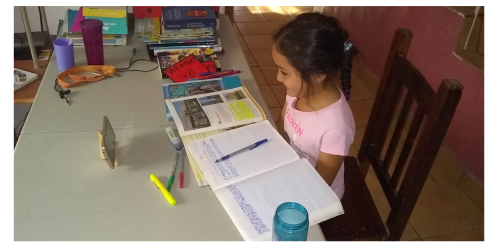
\includegraphics[width=0.45\textwidth]{Figs/LearningMonitoring3}
     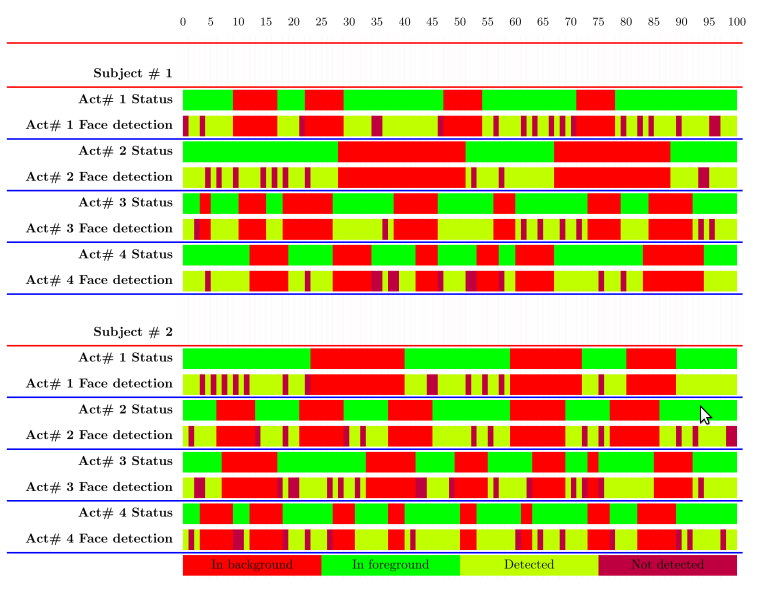
\includegraphics[width=0.80\textwidth]{Figs/LearningMonitoring4}

     \end{center}
\end{column}
\end{columns}

\end{block} 
\end{frame}

